%
% File tupa_multitask.tex

\documentclass[11pt,a4paper]{article}
\usepackage[hyperref]{acl2018}
\usepackage{times}
\usepackage{latexsym}
\usepackage{amsmath}
\usepackage{tikz}
\usepackage{tikz-dependency}
\usepackage[warn]{textcomp}
\usepackage{subcaption}
\usepackage{multirow}
\usepackage{url}
\usepackage{etoolbox}

\newcommand{\com}[1]{}
\newcommand{\oa}[1]{\footnote{\color{red}OA: #1}}

\hyphenation{SemEval}

\DeclareMathOperator*{\argmin}{argmin}
\DeclareMathOperator*{\argmax}{argmax}

\makeatletter
\patchcmd\@combinedblfloats{\box\@outputbox}{\unvbox\@outputbox}{}{%
   \errmessage{\noexpand\@combinedblfloats could not be patched}%
}%
 \makeatother


\usetikzlibrary{shapes,shapes.misc}

%\aclfinalcopy % Uncomment this line for the final submission
%\def\aclpaperid{***} %  Enter the acl Paper ID here

%\setlength\titlebox{5cm}
% You can expand the titlebox if you need extra space
% to show all the authors. Please do not make the titlebox
% smaller than 5cm (the original size); we will check this
% in the camera-ready version and ask you to change it back.

\title{Multitask Parsing across Semantic Representation Schemes}

\author{Daniel Hershcovich$^{1,2}$ \\
  \\\And
  Omri Abend$^2$ \\
  $^1$The Edmond and Lily Safra Center for Brain Sciences \\
  $^2$School of Computer Science and Engineering \\
  Hebrew University of Jerusalem \\
  \texttt{\{danielh,oabend,arir\}@cs.huji.ac.il}
  \\\And
  Ari Rappoport$^2$
}

\date{}

\begin{document}

\maketitle

\begin{abstract}
The ability to leverage and consolidate information of different types
is at the core of semantic learning, and is also practically appealing
in that it effectively extends the training data. In this paper we
tackle the challenging setting of improving semantic parsing
performance, taking other parsing tasks as auxiliaries. We take UCCA
parsing as a test case, and take AMR, SDP and Universal Dependencies
parsing as auxiliaries. We show that despite the notable conceptual
and formal differences between these schemes, they can all be
leveraged to improve UCCA parsing, using a flexible and uniform
parsing and learning architecture. We report substantial improvements
to UCCA parsing in both in-domain and out-domain settings, and across
three languages.
\end{abstract}

\section{Introduction}\label{sec:introduction}

The multitude of semantic representations put forth in recent years greatly enrich
the discussion in NLP on the nature of semantic structure.
Still, semantic representation has arguably yet to reach its full 
potential in terms of its contribution to downstream linguistic tasks,
partially due to the limited amounts of semantically annotated
corpora to train on. This shortage is even more pronounced in 
languages other than English, and less researched domains. 

%While the development of syntactic treebanks has had a tremendous impact on natural 
%language processing, semantic representation has arguably yet to reach its full 
%potential in terms of its contribution to downstream linguistic tasks.
%As an example for syntactic annotation, the Universal Dependencies (UD) project provides
%cross-linguistically consistent treebanks in many languages \cite{nivre2016universal},
%and accurate parsers based upon it and other datasets have been extremely useful in natural
%language understanding tasks \cite{P16-1139,E17-1117,K17-3002}.
%Semantic representation, while increasingly adopting whole-text annotation rather than more specific
%shallow schemes, faces several challenges: semantic distinctions, besides requiring deeper understanding
%and being harder to learn, are not always well-defined, and progress is hindered by fragmentation.
%Semantic schemes diverge in the content they choose to annotate, their coupling with syntax,
%and their degree of cross-linguistic applicability and consistency \cite{abend2017state}.

Indeed, recent work in semantic parsing has targeted, among others,
Abstract Meaning Representation \cite[AMR;][]{banarescu2013abstract,damonte-17,11099},
bilexical Semantic Dependencies \cite[SDP;][]{oepen2014semeval,oepen2015semeval,oepen2016towards,P17-1186}
with target representations such as DELPH-IN MRS \cite[DM;][]{flickinger2012deepbank},
and Universal Conceptual Cognitive Annotation \cite[UCCA;][]{abend2013universal,hershcovich2017a}.
While each of these schemes also focuses on a different set of distinctions,
much of the semantic content is shared \cite{abend2017state}.


%In cases where related tasks can be learned jointly,
%deep multitask learning models have been shown to be successful in various fields of NLP
%\cite{collobert2011natural,Zhang2016StackpropagationIR,P17-1186,swayamdipta2017frame,guo2016exploiting}.

We build on these ideas and propose a transition-based semantic DAG parser for UCCA,
trained in a multitask setting to obtain state-of-the-art 
results.\footnote{Our code is publicly available at $<$anonymized$>$.}

\begin{figure*}

\begin{subfigure}[t]{0.5\textwidth}
  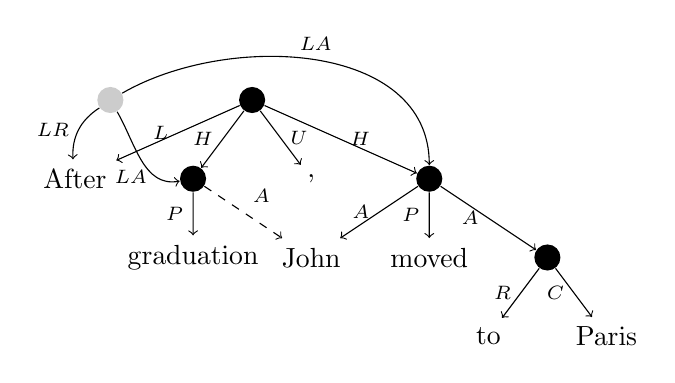
\begin{tikzpicture}[level distance=10mm, ->]
    \node (ROOT) [fill=black, circle] {}
      child {node (After) {After} edge from parent node[left] {\scriptsize $L$}}
      child {node (graduation) [fill=black, circle] {}
      {
        child {node {graduation} edge from parent node[left] {\scriptsize $P$}}
      } edge from parent node[left] {\scriptsize $H$} }
      child {node {,} edge from parent node[right] {\scriptsize $U$}}
      child {node (moved) [fill=black, circle] {}
      {
        child {node (John) {John} edge from parent node[left] {\scriptsize $A$}}
        child {node {moved} edge from parent node[left] {\scriptsize $P$}}
        child {node [fill=black, circle] {}
        {
          child {node {to} edge from parent node[left] {\scriptsize $R$}}
          child {node {Paris} edge from parent node[left] {\scriptsize $C$}}
        } edge from parent node[left] {\scriptsize $A$} }
      } edge from parent node[right] {\scriptsize $H$} }
      ;
    \draw[dashed,->] (graduation) to node [auto] {\scriptsize $A$} (John);
    \node (LKG) at (-1.8,0) [fill=black!20, circle] {};
    \draw[bend right] (LKG) to node [auto, left] {\scriptsize $LR$} (After);
    \draw (LKG) to[out=-60, in=190] node [below] {\scriptsize $LA\quad$} (graduation);
    \draw (LKG) to[out=30, in=90] node [above] {\scriptsize $LA$} (moved);
  \end{tikzpicture}
  \caption{UCCA \label{fig:original_example_ucca}}
\end{subfigure}
~
\begin{subfigure}[t]{0.5\textwidth}
  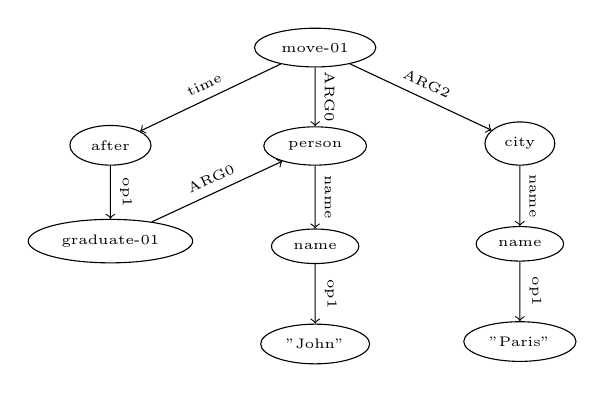
\begin{tikzpicture}[level distance=15mm, ->,
      every node/.append style={sloped,anchor=south,auto=false,font=\tiny},
      level 1/.style={sibling distance=26mm}]
    \node (ROOT) [draw=black,ellipse] {move-01}
      child {node [draw=black,ellipse] {after}
      {
            child {node (graduation) [draw=black,ellipse] {graduate-01} edge from parent node {op1} }
      } edge from parent node {time} }
      child {node (John) [draw=black,ellipse] {person}
      {
        child {node [draw=black,ellipse] {name}
        {
            child {node [draw=black,ellipse] {"John"} edge from parent node {op1} }
        } edge from parent node {name} }
      } edge from parent node {ARG0} }
      child {node [draw=black,ellipse] {city}
      {
        child {node [draw=black,ellipse] {name}
        {
            child {node [draw=black,ellipse] {"Paris"} edge from parent node {op1} }
        } edge from parent node {name} }
      } edge from parent node {ARG2} }
      ;
      \draw (graduation) to node {ARG0} (John);
  \end{tikzpicture}
  \caption{AMR \label{fig:original_example_amr}}
\end{subfigure}

\begin{subfigure}[t]{0.5\textwidth}
    \begin{dependency}[text only label, label style={above}, font=\small]
    \begin{deptext}[column sep=1em,ampersand replacement=\^]
    After \^ graduation \^ , \^ John \^ moved \^ to \^ Paris \\
    \end{deptext}
        \depedge{1}{2}{ARG2}
        \depedge{5}{4}{ARG1}
        \depedge[edge unit distance=2ex]{1}{5}{ARG1}
        \deproot{5}{top}
        \depedge[edge unit distance=4ex, edge start x offset=-1ex]{5}{7}{ARG2}
        \depedge[edge start x offset=1ex]{6}{5}{ARG1}
        \depedge{6}{7}{ARG2}
    \end{dependency}
  \caption{SDP \label{fig:original_example_sdp}}
\end{subfigure}
~
\begin{subfigure}[t]{0.5\textwidth}
    \begin{dependency}[text only label, label style={above}, font=\small]
    \begin{deptext}[column sep=1em,ampersand replacement=\^]
    After \^ graduation \^ , \^ John \^ moved \^ to \^ Paris \\
    \end{deptext}
        \depedge{2}{1}{case}
        \depedge{4}{3}{punct}
        \depedge{5}{4}{nsubj}
        \depedge{2}{5}{obl}
        \depedge{7}{6}{case}
        \deproot{5}{root}
        \depedge{5}{7}{obl}
    \end{dependency}
  \caption{UD \label{fig:original_example_ud}}
\end{subfigure}


\caption{\label{fig:original_examples}
 Example graph for each representation scheme we use.
 Figure \ref{fig:original_example_ucca} presents a UCCA graph. The dashed edge is remote,
  while the gray node and its outgoing edges represent inter-Scene linkage.
  Pre-terminal nodes and edges are omitted for brevity. 
 Figure \ref{fig:original_example_amr} presents an AMR graph.
  The text tokens are not part of the graph, and must be matched to
  concepts and constants by alignment. Variables are represented by their concepts.
 Figure \ref{fig:original_example_sdp} presents an SDP graph (in the DM formalism).
  The graph contains multiple roots: ``After'', ``moved'' and ``to''.
  One of the roots is marked as \textit{top}: ``moved''.
  Punctuation is not included in the graph as it is non-content-bearing.
 Figure \ref{fig:original_example_ud} presents a UD tree.
  Each word has exactly one head, and there is a single root.
  Edge labels correspond to syntactic relations.
}

\end{figure*}



%%%%%%%%%%%%%%%%%%%%%%%%%%%%%%%%%%%%%%%%%%%%%%%%%%%%%%%%%%%%%%%%%%%%%%%%%%%%%%%%%
\section{Related Work}\label{sec:related_work}

%In general, multitask learning involves optimizing more than one loss function \cite{ruder2017overview}.
%However, in our case, the loss function has the same form across all tasks.
%The same architecture and inference algorithm are applied to multiple annotation formats and datasets,
%and only some of the parameters are shared between them: this is hard parameter sharing.

\paragraph{Joint and multitask learning in NLP.}

These techniques have been used extensively in NLP,
for tasks with varying degrees of similarity and structure:
from joint semantic role labeling for different arguments of the same predicate
\cite{toutanova2005joint} to
joint syntactic and semantic parsing \cite{henderson2013multilingual}, to
incorporation of unlabeled data for various tasks \cite{ando2005framework}.
They are also used for domain adaptation in the same task \cite{W06-1615,P07-1033}.
Multitask learning can be used as regularization, or to enlarge the effective training data.
Joint learning is often used as an alternative to the pipeline approach,
alleviating cascading errors:
in transition-based parsing, it has been used for joint POS tagging and parsing \cite{bohnet2012transition}.

Representation learning has enabled much progress in multitask learning,
as it provides a straightforward way to share intermediate features between models:
for frame semantic parsing \cite{swayamdipta2017frame},
semantic dependency parsing for different target representations \citet{P17-1186} 
and domain adaptation \cite{K17-1040}, to name a few.
The whole NLP pipeline can even be replaced with a joint many-task model
\cite[JMT; ][]{collobert2011natural,D17-1206}.
However, we are not aware of a semantic parser using a single model for
widely different representation schemes.

In transition-based parsing, joint learning has also been applied to
tagging and parsing \cite{Zhang2016StackpropagationIR},
lexical and syntactic analysis \cite{constant-nivre:2016:P16-1,more2016joint},
syntactic and semantic parsing \cite{swayamdipta-EtAl:2016:CoNLL},
and multilingual parsing \cite{Q16-1031,guo2016exploiting}.

\paragraph{Transition-based semantic parsing.}

First used for projective syntactic dependency tree parsing
\cite{nivre2008algorithms},
subsequent work generalized transition-based parsing to non-projective and (discontinuous) constituency
parsing \cite{nivre2009non,zhang2009transition,maier-lichte:2016:DiscoNLP}.
Research on transition-based semantic dependency parsing and UCCA parsing
has introduced transitions to enable DAG parsing in general
\cite{sagae2008shift,ribeyre-villemontedelaclergerie-seddah:2014:SemEval,du-EtAl:2015:SemEval,hershcovich2017a}.
Transition-based AMR parsers either process dependency trees into AMRs
\cite{wang-xue-pradhan:2015:ACL-IJCNLP,wang2015transition,wang-EtAl:2016:SemEval,goodman2016noise},
or have a transition system tailored to AMR parsing \citet{zhou2016amr,damonte-17,D17-1130},
but we are not aware of a general transition-based DAG parser that handles AMR, too.



%%%%%%%%%%%%%%%%%%%%%%%%%%%%%%%%%%%%%%%%%%%%%%%%%%%%%%%%%%%%%%%%%%%%%%%%%%%%%%%%%
\section{Tackled Tasks}\label{sec:tasks}

In this section, we outline the parsing tasks we are addressing.
We focus on representation schemes that provide a \textit{full-sentence} analysis,
that is, schemes that produce a graph covering all (content) words in the text, or the
lexical concepts they evoke.
Full-sentence analysis contrasts with ``shallow'' semantic parsing,
primarily Semantic Role Labeling
\cite[SRL;][]{Palmer:05,gildea2002automatic,swayamdipta2017frame,ringgaard2017sling},
which target argument structure phenomena and uses flat structures.
We consider four target representations: UCCA, AMR, DM and UD
\cite[Universal Dependencies; ][]{nivre2016universal}.
Figure~\ref{fig:original_examples} shows an example graph for each scheme,
annotating the sentence ``After graduation, John moved to Paris''.

%Although each of these tasks uses different graph structures,
%they all involve whole-sentence (or whole-paragraph) semantic analysis,
%and due to the structure of phenomena such as predicate-argument relations,
%require parsers that can handle non-projectivity (or discontinuity) and reentrancy, resulting in
%directed acyclic graphs (DAGs).\oa{maybe add a diagram or at least elaborate more on these like we
%did in the TUPA paper, with examples etc.}

\paragraph{Universal Conceptual Cognitive Annotation.}\label{sec:ucca}
UCCA \cite{abend2013universal} is a semantic representation scheme whose main principles
are ease of annotation and cross-linguistic applicability and stability.
UCCA represents the semantics of natural language utterances
as directed acyclic graphs (DAGs), where terminal nodes (nodes without children)
correspond to the text tokens, and non-terminal nodes to semantic units that participate
in some super-ordinate relation.
Edges are labeled, indicating the role of a child in the relation the parent represents.
Nodes and edges may belong to one of several \textit{layers}, each corresponding
to a ``module'' of semantic distinctions.
UCCA's \textit{foundational layer} (the only layer for which annotated data exists) 
mostly covers predicate-argument structure, semantic heads and inter-Scene relations.
%The \textit{linkage} layer covers relations between events, including temporal and discourse relations
%(exemplified by the gray node and its outgoing edges in Figure~\ref{fig:original_example_ucca}).

UCCA's guidelines distinguish between \textit{primary} edges, corresponding 
to the roles explicit in the text, and \textit{remote} edges (such as the dashed edge in
Figure~\ref{fig:original_example_ucca}), corresponding to implicit relations.
Primary edges form a tree structure in each layer,
whereas remote edges enable reentrancy (a DAG structure).

As UCCA annotated data is currently quite scarce (see \S\ref{sec:data}), 
we hypothesize it will benefit from multitask learning, and consider it as our
main task.

%%%%%%%%%%%%%%%%%%%%%%%%%%%%%%%%%%%%%%%%%%%%%%%%%%%%%%%%%%%%%%%%%%%%%%%%%%%%%5
\paragraph{Abstract Meaning Representation.}\label{sec:amr}

AMR \cite{banarescu2013abstract}
is a semantic representation that encodes information about named entities, 
argument structure, semantic roles, word sense disambiguation and co-reference resolution.
AMRs are rooted directed graphs, in which both nodes and edges are labeled.
Most AMRs are DAGs, although cycles are permitted.
Despite the short time since its inception, AMR has been targeted by a number of works,
notably in the SemEval 2017 shared task \cite{may2017semeval}.

AMR differs from the other schemes considered here in that it does not anchor its graphs
in the words of the sentence (Figure~\ref{fig:original_example_amr}). Instead, AMR graphs
connect variables, concepts (from a pre-defined set) and constants (which may be strings or numbers).
Still, most AMR nodes are alignable to text tokens, a tendency used by AMR parsers,
which automatically align the graph nodes to the text in a process called \textit{concept identification}.
In this work, we use pre-aligned AMR graphs, which renders them (partially) anchored.


%%%%%%%%%%%%%%%%%%%%%%%%%%%%%%%%%%%%%%%%%%%%%%%%%%%%%%%%%%%%%%%%%%%%%%%%%%%%%5
\paragraph{Semantic Dependency Parsing.}\label{sec:sdp}

SDP is a set of related tasks, targeted in three recent SemEval shared tasks 
\cite{oepen2014semeval,oepen2015semeval,oepen2016towards}.
They correspond to four semantic representation schemes, referred to as
DM, PAS, PSD and CCD, representing
predicate-argument relations between content-bearing words in a sentence.
All are based on semantic formalisms whose annotations have been
converted into bilexical dependencies---labeled
directed graphs whose nodes are all text tokens.
Edges are labeled, encoding semantic relations between the tokens.
Non-content tokens, such as punctuation,
are often left out of the analysis (see Figure~\ref{fig:original_example_sdp}),
but the sub-graph restricted to content-bearing tokens is connected.
Graphs containing cycles have been removed from the SDP datasets.

We consider one of the three formalisms used in the SemEval shared tasks:
the DM (DELPH-IN MRS) representation, which comes
from DeepBank \cite{flickinger2012deepbank},
manually-corrected parses from the LinGO
English Resource Grammar \cite{copestake2000open}.
LinGO is a Head-driven Phrase
Structure Grammar \cite[HPSG; ][]{pollard1994head}
which uses Minimal Recursion Semantics \cite{copestake2005minimal}.

%%%%%%%%%%%%%%%%%%%%%%%%%%%%%%%%%%%%%%%%%%%%%%%%%%%%%%%%%%%%%%%%
\paragraph{Universal Dependencies.}\label{sec:ud}
UD \cite{nivre2016universal,11234/1-2515} is
the dominant dependency representation for
annotating treebanks in a large variety of languages,
aiming for cross-linguistically consistent and coarse-grained treebank
annotation. Formally, UD uses bilexical trees, with edge labels 
representing syntactic relations between words.

While not a semantic representation,
we use UD as an auxiliary task,
inspired by previous work on joint syntax and semantics
\cite{lluis2008joint,collobert2011natural,D15-1169,swayamdipta-EtAl:2016:CoNLL,swayamdipta2017frame}.
In order to obtain cross-linguistic applicability, 
UD often makes design decision that are similar to the common practice
in semantic treebanks, such as linking content words to content words wherever possible.
Moreover, using UD allows us to conduct experiments on French and German, 
for which SDP and AMR annotated data is not available (\S\ref{sec:multilingual}).

In addition to basic UD trees (such as in Figure~\ref{fig:original_example_ud}),
\textit{enhanced} and \textit{enhanced++} UD graphs are available for English,
using automatic converters included in Stanford CoreNLP \cite{SCHUSTER16.779}.
These include additional and augmented relations between content words,
partially overlapping with the notion of remote edges in UCCA:
in the case of control verbs, for example, a direct relation is added in enhanced UD
between the controlled verb and its controller,
which would likewise be represented by a remote edge in UCCA.

\begin{figure}[t]
   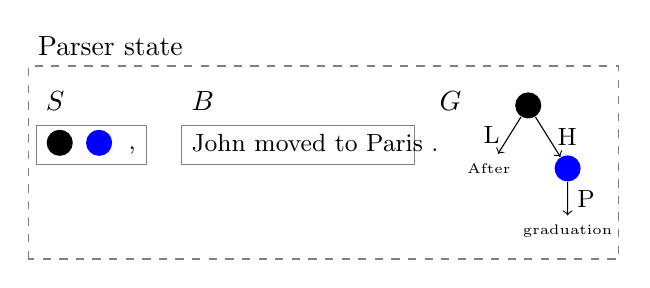
\begin{tikzpicture}[level distance=8mm, sibling distance=1cm]
   \node[anchor=west] at (0,1.5) {Parser state};
   \draw[color=gray,dashed] (0,-1.2) rectangle (7.5,1.25);
   \draw[color=gray] (.1,0) rectangle (1.5,.5);
   \node[anchor=west] at (.1,.8) {$S$};
   \node[fill=black, circle] at (.4,.275) {};
   \node[fill=blue, circle] at (.9,.275) {};
   \node[anchor=west] at (1.15,.175) {\small ,};
   \draw[color=gray] (1.95,0) rectangle (4.9,.5);
   \node[anchor=west] at (1.95,.8) {$B$};
   \node[anchor=west] at (1.95,.275) {\small John moved to Paris .};
   \node[anchor=west] at (5.1,.8) {$G$};
   \node[fill=black, circle] at (6.35,.75) {}
     child {node  {\tiny After} edge from parent [->] node[left] {\small L}}
     child {node [fill=blue, circle] {}
     {
       child {node {\tiny graduation} edge from parent [->] node[right] {\small P}}
     } edge from parent [->] node[right] {\small H} };
   \end{tikzpicture}
   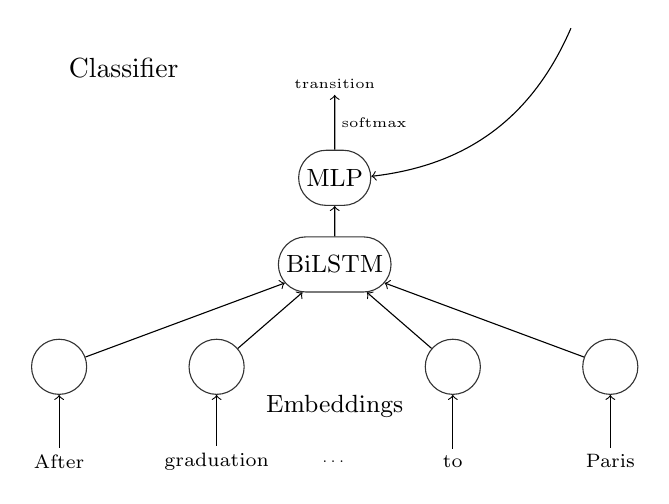
\begin{tikzpicture}[->]
   \node[anchor=west] at (0,6) {Classifier};
   \tiny
   \tikzstyle{main}=[rounded rectangle, minimum size=7mm, draw=black!80, node distance=12mm]
   \node[main] (specific) at (3.5,3.5) {\small BiLSTM};
   \node (embeddings) at (3.5,1.7) {\small Embeddings};
   \foreach \i/\word in {0/{After},2/{graduation},5/{to},7/{Paris}} {
       \node (x\i) at (\i,1) {\scriptsize \word};
       \node[main] (e\i) at (\i,2.2) {};
       \path (x\i) edge (e\i);
       \path (e\i) edge (specific);
   }
    \node (x4) at (3.5,1) {\ldots};
    \node[main] (mlp) at (3.5,4.6) {\small MLP};
    \path (specific) edge (mlp);
    \coordinate (state) at (6.5,6.5);
    \path (state) edge [bend left] (mlp);
    \node (transition) at (3.5,5.8) {transition};
    \path (mlp) edge node[right] {softmax} (transition);
   \end{tikzpicture}
\caption{Illustration of the TUPA model, adapted (with permission) from \citet{hershcovich2017a}.
Top: parser state.
Bottom: BiLTSM architecture.}
\label{fig:single_model}
\end{figure}


%%%%%%%%%%%%%%%%%%%%%%%%%%%%%%%%%%%%%%%%%%%%%%%%%%%%%%%%%%%%%%%%%%%%%%%%%%%%%%%%%%%%%%%%
\section{General Transition-based DAG Parser}\label{sec:model}

All tasks we outlined in \S\ref{sec:tasks} exhibit
reentrancy and discontinuity (or non-projectivity), to varying degrees.
In addition, UCCA and AMR contain non-terminal nodes.
In order to parse graphs with these structural properties,
we extend the TUPA parser \cite[][henceforth HAR17]{hershcovich2017a}, 
originally developed for UCCA parsing,
as it is the only parser to our knowledge that supports 
all these structural properties.
TUPA's transition system can yield any labeled DAG structure
whose leaves are aligned to text tokens.
To support parsing into AMR, which uses graphs that are not anchored in the tokens,
 we take advantage of existing alignments of the graphs with the text
tokens during training (\S\ref{sec:conversion}).

Transition-based parsers \cite{Nivre03anefficient} apply \textit{transitions}
incrementally to an internal state defined by a buffer $B$ of remaining tokens 
and nodes, a stack $S$ of incomplete nodes, and a labeled graph $G$ of 
constructed nodes and edges.
When the parsing process is finished, the graph $G$ is the final output.
A classifier is used at each step to select the next transition based on features
that encode the current state.
During training, an oracle creates training instances for the classifier,
based on gold-standard annotations.


\subsection{The Transition Set}\label{sec:transition_set}

Given a sequence of tokens $w_1, \ldots, w_n$,
we predict a rooted graph $G$ whose terminals are the tokens.
Parsing starts with the root node on the stack,
and the input tokens in the buffer.

The TUPA transition set includes
the standard \textsc{Shift} and \textsc{Reduce} operations,
\textsc{Node$_X$} for creating a new non-terminal node and an $X$-labeled edge,
\textsc{Left-Edge$_X$} and \textsc{Right-Edge$_X$} to create a new primary $X$-labeled edge,
\textsc{Left-Remote$_X$} and \textsc{Right-Remote$_X$} to create a new remote $X$-labeled edge,
\textsc{Swap} to handle discontinuous nodes,
and \textsc{Finish} to mark the state as terminal.

Although UCCA contains nodes without any text tokens as descendants
(named \textit{implicit units}),
these nodes are infrequent (about 0.5\% of non-terminal nodes), and
the standard evaluation for UCCA parsing is span-based and ignores them.
For this reason we follow HAR17 and do not include
any transition to create these when parsing UCCA,
thus ignoring them in both training and evaluation.
This phenomenon is even more common in AMR, as any unaligned concept
with no aligned descendents
will correspond to an implicit node (about 6\% of nodes).
These result from alignment errors, or from abstract concepts,
which have no explicit grounding in the text \cite{buys2017oxford}.
We ignore implicit nodes when training on AMR as well.

Another property of AMR not covered by TUPA is support for node labels, 
as only edges are labeled in UCCA. In AMR, however, node labels correspond 
to concepts and constants, and are ubiquitous.
When training on AMR, we produce graphs only with edge labels (relations) 
and without node labels.


%%%%%%%%%%%%%%%%%%%%%%%%%%%%%%%%%%%%%%%%%%%%%%%%%%%%%%%%%%%%%%%%%%%%%%%%%%%%%%%%%
\subsection{Transition Classifier}\label{sec:classifier}

To select the next transition at each time step,
we use a bidirectional LSTM with embeddings as inputs,
followed by a feedforward network and a softmax layer for classification 
(see Figure~\ref{fig:single_model}).
Inference is performed greedily,
and training is done with an oracle that yields the set of all correct 
transitions at a given state.
The network is trained to maximize the log-likelihood of all correct transitions at
each step, and the actual transition taken in training is the correct transition
with the highest score given by the classifier.


\begin{table}
\centering
\footnotesize
\begin{tabular}{l|c|ccccc}
\bf Hyperparameter &  \bf Single & \multicolumn{3}{c}{\bf Multitask} \\ 
&& \bf Main & \bf Aux & \bf Shared \\
\hline
external word dim. & 300 &&& 300 \\
word dim. & 200 &&& 200 \\
POS tag dim. & 20 &&& 20 \\
syntactic dep. dim. & 10 &&& 10 \\
named entity dim. & 3 &&& 3 \\
punctuation dim. & 1 &&& 1 \\
action dim. & 3 &&& 3 \\
edge label dim. & 20 & 20 & 20 \\
MLP layers & 2 & 2 & 1 \\
MLP dimensions & 50 & 50 & 50 \\
BiLSTM layers & 2 & 2 & 1 & 2 \\
BiLSTM dimensions & 500 & 250 & 50 & 250
\end{tabular}
\caption{Hyperparameter settings.\label{tab:hyperparams}
Middle column: single-task.
Right column: multitask settings for main task (UCCA), auxiliary tasks, and shared parameters.}
\end{table}

\begin{figure*}[t]
\begin{subfigure}{0.5\textwidth}
    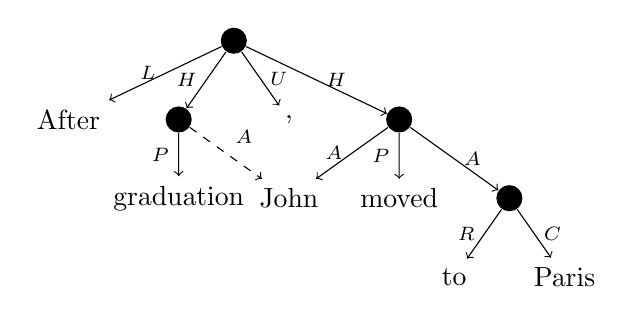
\begin{tikzpicture}[level distance=10mm, sibling distance=14mm, ->,
        every circle node/.append style={fill=black}]
      \tikzstyle{word} = [font=\rmfamily,color=black]
      \node (ROOT) [circle] {}
        child {node (After) [word] {After} edge from parent node[left] {\scriptsize $L$}}
        child {node (graduation) [circle] {}
        {
          child {node [word] {graduation} edge from parent node[left] {\scriptsize $P$}}
        } edge from parent node[left] {\scriptsize $H$} }
        child {node [word] {,} edge from parent node[right] {\scriptsize $U$}}
        child {node (moved) [circle] {}
        {
          child {node (John) [word] {John} edge from parent node[left] {\scriptsize $A$}}
          child {node [word] {moved} edge from parent node[left] {\scriptsize $P$}}
          child {node [circle] {}
          {
            child {node [word] {to} edge from parent node[left] {\scriptsize $R$}}
            child {node [word] {Paris} edge from parent node[right] {\scriptsize $C$}}
          } edge from parent node[right] {\scriptsize $A$} }
        } edge from parent node[right] {\scriptsize $H$} }
        ;
      \draw[dashed,->] (graduation) to node [auto] {\scriptsize $A$} (John);
    \end{tikzpicture}
  \caption{Converted UCCA graph.
  Linkage nodes and edges are removed, but the original graph is otherwise preserved.}
  \label{fig:converted_example_ucca}
\end{subfigure}
~
\begin{subfigure}{0.5\textwidth}
  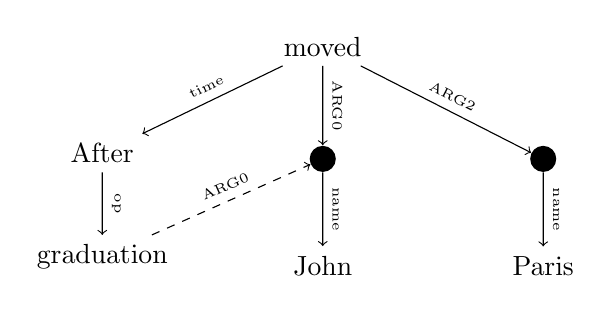
\begin{tikzpicture}[level distance=16mm, ->,
      every node/.append style={sloped,anchor=south,auto=false,font=\tiny},
      level 1/.style={sibling distance=28mm},
      level 2/.style={sibling distance=14mm},
      level 3/.style={sibling distance=12mm}]
    \tikzstyle{word} = [font=\rmfamily,color=black]
    \node (ROOT) [word] {moved}
      child {node [word] {After}
      {
            child {node (graduation) [word] {graduation} edge from parent node {op} }
      } edge from parent node {time} }
      child {node (John) [fill=black,circle] {}
      {
        child {node [word] {John} edge from parent node {name} }
      } edge from parent node {ARG0} }
      child {node [fill=black,circle] {}
      {
        child {node [word] {Paris} edge from parent node {name} }
      } edge from parent node {ARG2} }
      ;
      \draw[dashed] (graduation) to node {ARG0} (John);
  \end{tikzpicture}
  \captionof{figure}{Converted AMR graph, with
  text tokens added according to the alignments.
  Numeric suffixes of \textit{op} relations were removed,
  and names collapsed.}
  \label{fig:converted_example_amr}
\end{subfigure}

\begin{subfigure}{0.5\textwidth}
  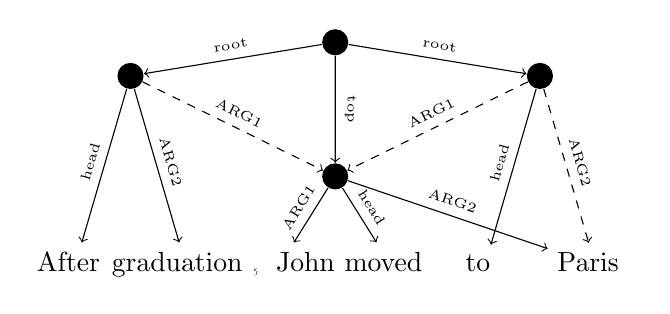
\begin{tikzpicture}[level distance=12mm, ->,
      every node/.append style={sloped,anchor=south,auto=false,font=\tiny},
      level 1/.style={sibling distance=26mm,level distance=6mm},
      level 2/.style={sibling distance=14mm,level distance=14mm}]
    \tikzstyle{word} = [font=\rmfamily,color=black]
    \node (ROOT) [fill=black,circle] {}
      child {node (after) [fill=black,circle] {}
      {
        child {node [draw=none] {}
        {
          child {node [word] (after_word) {After{\color{white}g}} edge from parent [draw=none]}
        } edge from parent [draw=none] }
        child {node [draw=none] {}
        {
          child {node [word] (graduation) {graduation ,} edge from parent [draw=none]}
        } edge from parent [draw=none] }
      } edge from parent node {root}}
      child {node [draw=none] {}
      {
        child {node (moved) [fill=black,circle] {}
        {
          child {node [word] {\quad{\color{white}g} John} edge from parent node {ARG1}}
          child {node [word] {moved{\color{white}g}} edge from parent node {head}}
        } edge from parent [draw=none] }
      } edge from parent [draw=none] }
      child {node (to) [fill=black,circle] {}
      {
        child {node [draw=none] {}
        {
            child {node [word] (to_word) {to{\color{white}g}} edge from parent [draw=none]}
          } edge from parent [draw=none] }
          child {node [draw=none] {}
        {
          child {node [word] (Paris) {Paris{\color{white}g}} edge from parent [draw=none]}
        } edge from parent [draw=none] }
      } edge from parent node {root}}
      ;
      \draw (ROOT) to node {top} (moved);
      \draw (after) to node {head} (after_word);
      \draw (after) to node {ARG2} (graduation);
      \draw[dashed] (after) to node {ARG1} (moved);
      \draw[dashed] (to) to node {ARG1} (moved);
      \draw (to) to node {head} (to_word);
      \draw (moved) to node {ARG2} (Paris);
      \draw[dashed] (to) to node {ARG2} (Paris);
  \end{tikzpicture}
  \captionof{figure}{Converted SDP graph (in the DM formalism), with
  intermediate non-terminal nodes introduced as \textit{head} units.
  In case of reentrancy, an arbitrary reentrant edge is marked as remote.}
  \label{fig:converted_example_sdp}
\end{subfigure}
~
\begin{subfigure}{0.5\textwidth}
  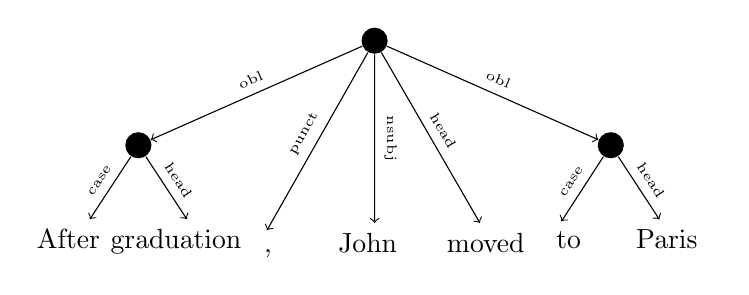
\begin{tikzpicture}[level distance=15mm, ->,
      every node/.append style={sloped,anchor=south,auto=false,font=\tiny},
      level 1/.style={sibling distance=15mm},
      level 2/.style={sibling distance=16mm}]
    \tikzstyle{word} = [font=\rmfamily,color=black]
    \node (ROOT) [fill=black,circle] {}
      child {node (after) [fill=black,circle] {}
      {
        child {node [word] {After{\color{white}g}} edge from parent node {case}}
        child {node [word] {graduation {\color{white}g}\quad\quad} edge from parent node {head}}
      } edge from parent node {obl}}
      child {node {}
      {
        child {node [word] (comma) {{\color{white}g} ,} edge from parent [draw=none]}
      } edge from parent [draw=none]}
      child {node {}
      {
        child {node [word] (John) {John{\color{white}g}} edge from parent [draw=none]}
      } edge from parent [draw=none]}
      child {node {}
      {
        child {node [word] (moved) {moved{\color{white}g}} edge from parent [draw=none]}
      } edge from parent [draw=none]}
      child {node (to) [fill=black,circle] {}
      {
          child {node [word] {\quad{\color{white}g}to} edge from parent node {case}}
          child {node [word] {Paris{\color{white}g}} edge from parent node {head}}
      } edge from parent node {obl}}
      ;
      \draw (ROOT) to node {punct} (comma);
      \draw (ROOT) to node {nsubj} (John);
      \draw (ROOT) to node {head} (moved);
  \end{tikzpicture}
  \captionof{figure}{Converted UD graph.
  As in SDP, intermediate non-terminals and \textit{head} edges are introduced.
  The graph is actually a tree, as was the original bilexical graph.}
  \label{fig:converted_example_ud}
\end{subfigure}

\caption{Unified DAG format
(pre-terminals omitted: each terminal drawn in place of its parent).}
\label{fig:converted_examples}
\end{figure*}


\paragraph{Features.}
In addition to the features used by HAR17,
representing the words, POS tags, syntactic dependency relations, and previously predicted edge labels
for nodes in specific locations in the parser state, for each token
we use feature embeddings representing the lemma, prefix, suffix, shape, and named entity type,
extracted using spaCy \cite{spacy2}.\footnote{\url{https://spacy.io}}
%For AMR we add node label features according to gold node labels.


\paragraph{Constraints.}
As each annotation scheme has different constraints on the allowed graphs,
we defined these constraints separately for each task.
During training and parsing, the constraint set corresponding to the task is
selected and applied to the parser state, to rule out some of the transitions.

Some constraints are task-specific, while some are generic.
For example, in UCCA, a terminal may only have one parent.
In AMR, a concept corresponding to a PropBank frame may only have 
core arguments defined for the frame.
An example of a generic constraint is that nodes on the stack 
that have already been swapped
should never be swapped again.\footnote{
	To implement this constraint, we define a \textit{swap index}
	for each node, which is assigned when the node is created.
	At parse start, only the root node and terminals exist.
	We assign the root a swap index of 0, and for each terminal, its swap index
	is its position in the text (starting at 1).
	Whenever a node is created as a result of a \textsc{Node}
	transition, we assign its swap index to be the arithmetic 
	mean of the stack top and buffer head's swap indices.}


%%%%%%%%%%%%%%%%%%%%%%%%%%%%%%%%%%%%%%%%%%%%%%%%%%%%%%%%%%%%%%%%%%%%%%%%%%%%%%%%%%%%%%%%
\section{Unified DAG Format}\label{sec:conversion}

To be able to use TUPA for the four tasks presented in \S\ref{sec:tasks},
we convert them all into a unified DAG format, which is inclusive enough to
allow representing any of the schemes with very little loss of information.

The format consists of a rooted DAG, where the tokens are the terminal nodes.
As in the UCCA format, the edges (but not the nodes) are labeled,
and are divided into \textit{primary} and \textit{remote} edges,
where the primary edges form a tree (all nodes have at most one primary parent,
and the root has none).
The remote edges enable reentrancy, and thus together with them the graph
is generally a DAG, and not necessarily a tree.
Figure~\ref{fig:converted_examples} shows examples for converted graphs.
Converting UCCA into the unified format consists simply of removing linkage 
nodes and edges (see Figure~\ref{fig:converted_example_ucca}), which were
also discarded by HAR17.

\paragraph{Converting bilexical dependencies.}
In order to convert DM and UD into the unified DAG format,
we add a pre-terminal for each token,
and then attach the pre-terminals according to the original dependency edges:
traversing the tree from the root down, for each head token we create a non-terminal
parent with the edge label {\it head},
and add the node's dependents as children of the created non-terminal node
(see Figures~\ref{fig:converted_example_sdp} and \ref{fig:converted_example_ud}).
Since DM allows multiple roots, we form a single root node, whose children
are the original roots. The added edges are labeled \textit{root}, where
top nodes are labeled \textit{top} instead.
In case of reentrancy, an arbitrary parent is marked as primary, and the rest as remote
(denoted as dashed edges in Figure~\ref{fig:converted_examples}).

\paragraph{Converting AMR.}
In the conversion from AMR, non-terminals are already present, and node labels are dropped.
However, alignments must be handled (see Figure~\ref{fig:converted_example_amr}).
Since alignment between nodes and text tokens is not part of the AMR graph,
we insert the alignments into the graph as edges in the conversion.
Specifically, we use automatically aligned graphs provided in the AMR dataset (see \S\ref{sec:data}),
and attach each node with a \textit{Terminal} edge to each of the terminals it is aligned to.
%
%Since the order of AMR ordinal relations, such as \textit{op1}, \textit{op2},
%is annotated according to the order of text tokens,
%the numeric index is redundant and is thus removed.
%Numeric suffixes are kept when they are meaningful, e.g. in distinguishing between PropBank semantic
%roles (\textit{ARG[0-5]}).

A named entity in AMR is represented as a sub-graph, whose \textit{name}-labeled root
has a child for each token in the name
(see the two \textit{name} nodes in Figure~\ref{fig:original_example_amr}).
We collapse this sub-graph into a single node whose children are the name tokens.


\begin{figure}[t]
   \begin{tikzpicture}
   \node[anchor=west] at (0,1.25) {Parser state};
   \draw[color=gray,dashed] (0,0) rectangle (7.5,1);
    \node (x4) at (3.75,0.5) {\ldots};
   \end{tikzpicture}
   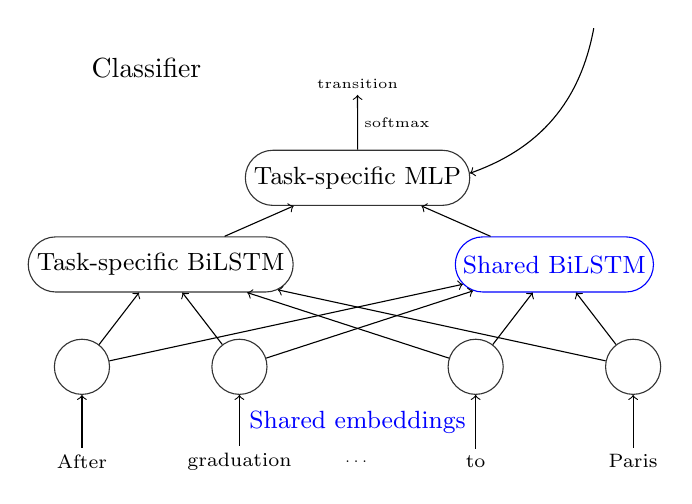
\begin{tikzpicture}[->]
   \node[anchor=west] at (0,6) {Classifier};
   \tiny
   \tikzstyle{main}=[rounded rectangle, minimum size=7mm, draw=black!80, node distance=12mm]
   \node[main] (specific) at (1,3.5) {\small Task-specific BiLSTM};
   \node[main,color=blue] (shared) at (6,3.5) {\small Shared BiLSTM};
   \node[color=blue] (embeddings) at (3.5,1.5) {\small Shared embeddings};
   \foreach \i/\word in {0/{After},2/{graduation},5/{to},7/{Paris}} {
       \node (x\i) at (\i,1) {\scriptsize \word};
       \node[main] (e\i) at (\i,2.2) {};
       \path (x\i) edge (e\i);
       \path (e\i) edge (specific);
       \path (e\i) edge (shared);
   }
    \node (x4) at (3.5,1) {\ldots};
    \node[main] (mlp) at (3.5,4.6) {\small Task-specific MLP};
    \path (specific) edge (mlp);
    \path (shared) edge (mlp);
    \coordinate (state) at (6.5,6.5);
    \path (state) edge [bend left] (mlp);
    \node (transition) at (3.5,5.8) {transition};
    \path (mlp) edge node[right] {softmax} (transition);
   \end{tikzpicture}
   \caption{Multitask model.
      Representations for input tokens are computed by two BiLSTMs:
      a task-specific one and a share one. The result is concatenated with
      features from the parser state and fed into the MLP for selecting the next transition.}
   \label{fig:multi_model}
\end{figure}

\begin{table*}[ht]
\centering
\begin{tabular}{ll|rr|rr|rr}
& & \multicolumn{2}{c|}{\footnotesize \bf English} & \multicolumn{2}{c|}{\footnotesize \bf French} & \multicolumn{2}{c}{\footnotesize \bf German} \\
\multicolumn{2}{c|}{\footnotesize \bf Corpus} & \footnotesize \bf {\#}tok & \footnotesize \bf {\#}sent & \footnotesize \bf {\#}tok & \footnotesize \bf {\#}sent & \footnotesize \bf {\#}tok & \footnotesize \bf {\#}sent \\
\hline
\textbf{UCCA}
& Wiki & 158433 & 5225 &&&& \\
& 20K Leagues & 12339 & 506 & 12929 & 547 & 113524 & 4764 \\
\hline
\textbf{UD} & v2.1 & 568560 & 24276 & 540942 & 21567 & 318847 & 16590 \\
\hline
\textbf{AMR} & LDC2017T10 & 708701 & 39260 \\
\hline
\textbf{DM} & SDP 2016 & 802717 & 35657 \\
\end{tabular}
\caption{Size of each corpus: total number of tokens ({\#}tok) and sentences
({\#}sent).\label{tab:corpora}}
\end{table*}


%%%%%%%%%%%%%%%%%%%%%%%%%%%%%%%%%%%%%%%%%%%%%%%%%%%%%%%%%%%%%%%%%%%%%%%%%%%%%%%%%%%%%%%%%%%%
\section{Multitask Transition-based Parsing}\label{sec:multitask}

Since the same TUPA model can be applied to different tasks, 
we can train it on multiple tasks together.
Following previous work, we use similar hyperparameter settings as for the single-task 
case (see Table~\ref{tab:hyperparams}, right column),
and rather than sharing all model parameters, share only part of the model
\cite{N16-1179,P16-2038,C16-1013,C16-1059,C16-1179,E17-1005,P17-1186}:
feature embeddings are shared, and in addition to the task-specific BiLSTM,
we use a shared BiLSTM. The outputs of both BiLSTMs are concatenated and
fed into the task-specific MLP (see Figure~\ref{fig:multi_model}).

The fairly small training set available for UCCA (see \S\ref{sec:data})
makes multitask learning particularly appealing,
and we focus on it in this paper, treating AMR, DM and UD parsing as auxiliary tasks.

\paragraph{Unlabeled parsing for auxiliary tasks.}

To simplify the auxiliary tasks and facilitate generalization \cite{E17-2026},
we perform unlabeled parsing for AMR, DM and UD in the multitask setting,
while still predicting edge labels in UCCA parsing.
We extend TUPA to support unlabeled parsing by simply removing all labels from the
\textsc{Edge}, \textsc{Remote} and \textsc{Node} transitions outputted by the oracle.
This results in a much smaller output dimension,
and we use a smaller task-specific BiLSTM for the auxiliary tasks.\oa{what do you mean?
		that because there are less transitions you need less states in the BiLSTM? if so, write
		it this way}



\section{Experiments}\label{sec:experiments}

We perform various experiments to evaluate the benefit of each auxiliary task to UCCA parsing.
First, we train the parser only on UCCA, and evaluate its performance.
Next, we train it in a multitask setting, where AMR, DM and UD are used as
auxiliary tasks.

\subsection{Data}\label{sec:data}

For UCCA, we use the English Wikipedia corpus \cite{abend2013universal},
with the standard train/dev/test split of 4254/453/518 sentences.
In addition, we use
the \textit{Twenty Thousand Leagues Under the Sea} corpus \cite[20K leagues;][]{sulem2015conceptual},
annotated in English, French and German.
The English part is used only for testing.
Due to their small size, and since they are still under development, we only use a train/dev split
in the French and German datasets, of 480/67 and 4196/561 sentences, respectively.
We report results on the development set for these datasets.\footnote{UCCA corpora are publicly
available at $<$anonymized$>$}

For AMR, we use LDC2017T10, targeted in SemEval 2017
\cite{may2017semeval}.\footnote{\url{https://catalog.ldc.upenn.edu/LDC2017T10}}
For SDP, we use the DM target representation from the SDP 2016 dataset
\cite{oepen2016towards}.\footnote{\url{http://sdp.delph-in.net/osdp-12.tgz}}
For Universal Dependencies, we use all English, French and German treebanks from UD v2.1
\cite{11234/1-2515}.\footnote{\url{http://hdl.handle.net/11234/1-2515}}
We use the enhanced++ UD representation \cite{SCHUSTER16.779} in our English experiments,
henceforth referred to as UD$^{++}$.
Table~\ref{tab:corpora} shows the size of each corpus.

Training proceeds by creating a unified corpus by shuffling all sentences from relevant
datasets together (according to the setting),
but using only the score on the UCCA development set as the criterion for early stopping.
In each training epoch, we use the same number of examples from each task.
Since the training sets are different in size, we sample the same number of sentences from
the training set of each of the other tasks.\oa{how many in each iteration?}

\begin{table*}
\centering
\begin{tabular}{l|ccc|ccc||ccc|ccc}
& \multicolumn{6}{c||}{\footnotesize \bf Wiki (in-domain)}
& \multicolumn{6}{c}{\footnotesize \bf 20K Leagues (out-of-domain)} \\
& \multicolumn{3}{c|}{\footnotesize \bf Primary} & \multicolumn{3}{c||}{\footnotesize \bf Remote}
& \multicolumn{3}{c|}{\footnotesize \bf Primary} & \multicolumn{3}{c}{\footnotesize \bf Remote} \\
& \footnotesize \textbf{LP} & \footnotesize \textbf{LR} & \footnotesize \textbf{LF}
& \footnotesize \textbf{LP} & \footnotesize \textbf{LR} & \footnotesize \textbf{LF}
& \footnotesize \textbf{LP} & \footnotesize \textbf{LR} & \footnotesize \textbf{LF}
& \footnotesize \textbf{LP} & \footnotesize \textbf{LR} & \footnotesize \textbf{LF} \\
\hline
Single-task
& 74.3 & 72.8 & 73.5 & 53 & 50 & 51.5 & 68.9 & 68.9 & 68.9 & 40.7 & 19.6 & 26.5 \\
\hline
\small \bf Multitask &&&&&&&&& \\
AMR \\
DM \\
UD$^{++}$ \\
AMR + DM \\
AMR + UD$^{++}$ \\
DM + UD$^{++}$ \\
AMR + DM + UD$^{++}$ 
\end{tabular}
\caption{
Experimental results, in percents, on the English \textit{Wiki} test set (left)
and \textit{20K Leagues} set (right).
Columns correspond to labeled precision, recall and F-score,
for both primary and remote edges.
}
\label{tab:results}
\end{table*}


\subsection{Evaluation}\label{sec:evaluation}

%As each scheme has its own evaluation metric, we evaluate them separately.
We evaluate on UCCA using labeled precision, recall and F1 on primary and remote edges,
following previous work on UCCA parsing \cite{hershcovich2017a}.
Edges in predicted and gold graphs are matched by terminal yield and label.
%For UD, we use LAS F1.
%For AMR, we use Smatch \cite{cai2013smatch}.
%For DM, we use labeled precision, recall and F1.



\subsection{Training}

All embeddings are initialized randomly.
For words, we additionally use external word embeddings containing 250K word vectors from fastText
\cite{bojanowski2016enriching},\footnote{\url{https://github.com/facebookresearch/fastText}}
pre-trained over Wikipedia and updated during training.
We use dropout \cite{srivastava2014dropout} between MLP layers and recurrent dropout
\cite{NIPS2016_6241} between BiLSTM layers, both with a probability of 0.4.
In addition, we use word, tag and dependency relation dropout \cite{kiperwasser2016simple}:
in training, the embedding for a feature value $w$ is replaced with a zero vector
with a probability of $\frac{0.2}{\#(w)+0.2}$, where $\#(w)$ is the number of occurrences of the
$w$ observed so far.
For optimization we a minibatch size of 100, decaying all weights by $10^{-5}$ at each update,
and train with stochastic gradient descent (SGD) for 40 epochs with a learning
rate of 0.1, followed by AMSGrad \cite{j.2018on} for 60 epochs with
$\alpha=0.001,\beta_1=0.9,\beta_2=0.999$.
We found this training strategy to work better than using only one of the optimization methods,
similar to findings by \citet{keskar2017improving}.
We select the epoch with the best labeled F1 score on the development set.
The neural network is implemented using DyNet \cite{neubig2017dynet}.\footnote{\url{https://dynet.io}}
Hyperparameter settings are listed in Table~\ref{tab:hyperparams} (middle column).

\subsection{Ensembling}

During inference, we use Product of Experts \cite[PoE; ][]{hinton2002training} to combine the predictions
of three models trained in the same setting, but with different random seeds. The transition selected is
\[
\argmax_{t\in T}\sum_{i=1}^3\big[\log(\mathrm{softmax}(m_i(s)))\big]_t
\]
where $T$ is the set of possible transitions, $m_i$ are the combined models, and $s$ is the current state.

In order to ensemble multitask models, we combine models trained with the same auxiliary task.
Another alternative is to combine models trained with different auxiliary tasks.\oa{don't write about alternatives,
but rather on what we actually do}
This provides greater variability between the combined models.



\subsection{Results}\label{sec:results}

%\subsection{Single-task parsing}\label{sec:results_single}
%
%To evaluate the conversion and parsing algorithm on each task, we report the result
%of training the parser on each task separately.
%In this case we perform labeled parsing for all tasks, and use the whole training set.
%The results for single-task parsing, when evaluated on the development set for each task,
%are shown in Table~\ref{tab:single}.
%
%
%
%\begin{table}
%\centering
%\begin{tabular}{l|ccc}
%\textbf{UD English} && \multicolumn{2}{r}{\textbf{LAS F1}} \\
%Ours &&& 80.1 \\
%D\&M &&& 82.2 \\
%\hline
%\textbf{AMR} & \textbf{P} & \textbf{R} & \textbf{F1} \\
%Ours & 66.7 & 64.7 & 65.7 \\
%F\&M &&& 70.9 \\
%\hline
%\textbf{DM} & \textbf{LP} & \textbf{LR} & \textbf{LF} \\
%Ours & 76 & 75.4 & 75.7 \\
%CMU &&& 89.4
%\end{tabular}
%\caption{Single-task results on dev set for each auxiliary task,
%when trained only on that task.
%Best reported results given for comparison:
%D\&M is \citet{dozat2016deep},
%F\&M is \citet{foland2017abstract},
%and CMU is \citet{thomson-EtAl:2014:SemEval}.
%AMR is evaluated by Smatch \cite{cai2013smatch}.
%\label{tab:single}}
%\end{table}

%\subsection{Multitask parsing}\label{sec:results_multi}

Table~\ref{tab:results} shows our main experimental results.
Our basic single-task model is comparable to \citet{hershcovich2017a}, as it is using a similar model.
%Our basic single-task model already outperforms the previous state of the art on
%UCCA parsing \cite{hershcovich2017a}, gaining a 2\% error reduction on in-domain primary labeled F1,
%and comparable results on remote edges.
%This improvement can be attributed to ensembling,
%as our model is otherwise similar to the one of \citet{hershcovich2017a}.


\subsection{Other languages}\label{sec:multilingual}

To investigate the contribution of multitask training on an even smaller UCCA training set,
we experiment with the French and German \textit{20K Leagues} UCCA corpora
\cite{sulem2015conceptual}
in a single-task and multitask setting, where as an auxiliary task we use unlabeled parsing on
UD treebanks in the respective languages.\footnote{We did not use AMR, DM or enhanced UD in French
and German, as these are only available in English.}
The results are given in Table~\ref{tab:multilingual}.
The contribution of multitask learning is substantial in this case:
11\% error reduction on the French dataset, and 1.5\% on the larger German dataset
(see Table~\ref{tab:corpora}).
This result demonstrates that even a small training set in the main task may produce good results,
given a sufficiently large training set for an auxiliary task.

\begin{table}
\begin{tabular}{l|ccc|ccc}
& \multicolumn{3}{c|}{\footnotesize \bf Primary} & \multicolumn{3}{c}{\footnotesize \bf Remote} \\
& \footnotesize \textbf{LP} & \footnotesize \textbf{LR} & \footnotesize \textbf{LF}
& \footnotesize \textbf{LP} & \footnotesize \textbf{LR} & \footnotesize \textbf{LF} \\
\hline
\multicolumn{4}{l|}{\small \bf French} & \\
\small Single & 59.4 & 59.8 & 59.6 & 5.9 & 1.9 & 2.9 \\
\small Multi & 66.1 & 66.2 & 66.2 & 33.3 & 9.4 & 14.7 \\
\hline
\multicolumn{4}{l|}{\small \bf German} & \\
\small Single & 73.7 & 72.4 & 73.1 & 49.2 & 12.3 & 19.7 \\
\small Multi & 74.6 & 73.7 & 74.2 & 61.7 & 20.6 & 30.9
\end{tabular}
\caption{Results on the UCCA \textit{20K Leagues}
development set in French and German.
\textit{Single} is trained only on the corresponding UCCA training set,
while \textit{Multi} uses unlabeled UD parsing in the same language as an auxiliary task.
\label{tab:multilingual}}
\end{table}

\begin{table}
\begin{tabular}{l|ccc|ccc}
& \multicolumn{3}{c|}{\footnotesize \bf Primary} & \multicolumn{3}{c}{\footnotesize \bf Remote} \\
& \footnotesize \textbf{UP} & \footnotesize \textbf{UR} & \footnotesize \textbf{UF}
& \footnotesize \textbf{UP} & \footnotesize \textbf{UR} & \footnotesize \textbf{UF} \\
\hline
AMR & 52.2 & 15.5 & 23.9 & 7.3 & 5.5 & 6.3 \\
DM & 63.6 & 49.8 & 55.9 & 6.9 & 63.8 & 12.4 \\
%UD & 75.3 & 82.9 & 78.9 & -- & 0 & -- \\
%UD$^+$ & 75.1 & 82.4 & 78.5 & 11.5 & 12.8 & 12.1 \\
UD$^{++}$ & 75.1 & 82.5 & 78.6 & 11.8 & 12.8 & 12.2
\end{tabular}
\caption{Unlabeled UCCA evaluation of 100 sentences converted to the unified DAG format.
\label{tab:common}}
\end{table}


\section{Discussion}\label{sec:discussion}

An important factor in the success of multitask learning is the commonalities between the tasks
\cite{E17-2026,E17-1005}.
%In fact, this is why we decided to convert the auxiliary tasks into UCCA-like format for
%multitask training in the first place.
To evaluate the similarity between the unlabeled auxiliary tasks and UCCA parsing,
we perform unlabeled evaluation of a manually annotated sample of 100 sentences from the
Wall Street Journal, after conversion to the unified DAG format.\footnote{The annotated
sentences are available at $<$anonymized$>$}
As can be seen in Table~\ref{tab:common}, there is a high unlabeled overlap between
UCCA and UD$^{++}$ after conversion to the unified DAG format,
while AMR is much less similar.
DM contains a fair amount of information about primary UCCA edges, and even more about remote edges.

These findings correlate with our multitask experimental results:
while using AMR as an auxiliary task did not contribute much, DM and UD$^{++}$ did benefit UCCA
parsing, and their combination yielded an even greater improvement.

While we focus on UCCA parsing in this work, our parser is capable of parsing any
scheme that can be represented in the unified DAG format.
This is a step towards general AI: a single model that can handle many different tasks.
Preliminary experiments using a similar architecture to the one presented in this paper have produced
promising results on each of the tasks' respective development sets:
67.1\% Smatch F1 \cite{cai2013smatch} on AMR
(using additional transitions and classifier for node labels and implicit nodes),
76.5\% labeled F1 on SDP (DM),
and 80.1\% LAS F1 on UD (English).
For AMR and UD, these are not far from the state-of-the-art results on these datasets
\cite{foland2017abstract,dozat2016deep}.
In future work, we plan to pursue this direction further and investigate whether a single
algorithm and architecture can be competitive on all of these parsing tasks.

\section{Conclusion}


\bibliography{references}
\bibliographystyle{acl_natbib}

\end{document}
